\documentclass[a4paper,11pt,titlepage]{article}
\usepackage[utf8]{inputenc}
\usepackage[czech]{babel}
\usepackage{amsmath}
\usepackage{xcolor}
\usepackage{subcaption}
\usepackage[top=48pt,bottom=48pt,left=48pt,right=48pt]{geometry}
\title{\textbf{SEN: Černá skříňka pro automobil}}
\author{Petr Rusiňák (xrusin03), Andrej Hučko (xhucko01)}
\date{Říjen 2018}
\usepackage{graphicx}
\usepackage{makecell}
\usepackage[hidelinks]{hyperref}
\usepackage{listings}

\begin{document}

\maketitle


\section{Úvod}

Cílem tohoto projektu je vytvořit jednoduchou „černou skříňku“ pro automobil, která
v~případě detekce nárazu odešle prostřednictvím Bluetooth informaci o~poloze vozidla
a~síle nárazu na server. Na serveru bude spuštěna aplikace, která tyto získané přijaté údaje
zobrazí.

\section{Použité zařízení a~technologie}

Vlastní černá skříňka je realizována kitem \href{https://www.st.com/en/evaluation-tools/nucleo-f446re.html}{STM32 Nucleo 446RE}, který složí jako mikrokontrolér,
senzory pro zjištění vstupních veličin (zrychlení a~poloha) a~Bluetooth modulem pro komunikaci se serverem.
Konkrétně se jedná o~akcelerometr
\href{https://www.pololu.com/product/2127}{Pololu LSM303D}, GPS senzor \href{https://www.u-blox.com/en/product/neo-6-series}{u-blox NEO 6M} a~Bluetooth modul \href{http://wiki.keyestudio.com/index.php/Ks0055_keyestudio_Bluetooth_Module}{Keyestudio Ks0055 HC-06}.
Ke komunikaci mezi kitem a~akcelerometrem se používá rozhraní I2C, zatímco GPS a~Bluetooth moduly
s~kitem komunikují pomocí sériového rozhraní.

Serverová část je řešena jako aplikace pro Android, která může pomocí Bluetooth jednoduše
komunikovat s~kitem dle zpráv popsaných v~kapitole \ref{msgs}.

\section{Schéma připojení periferií ke kitu}

Na následujícím obrázku je znázorněno schéma zapojení periferií ke kitu STM32 Nucleo.
Všechna zařízení jsou napájena napětím 3,3 V~a~připojena k~zemi. Bluetooth modul
je připojen pomocí sériové linky na UART1 (piny D2 a~D8). Pro obsloužení GPS modulu
postačuje pouze jednosměrná komunikace směrem do kitu, stačí tedy připojit
výstupní vodič senzoru k~vstupnímu pinu UART4 A1.~Vodiče akcelerometru SDA a~SCL
budou připojeny k~pinům kitu D14 a~D15 a~dále je nutné na vstup akcelerometru SDO přivést
logickou 0, čímž bude povolena komunikace pomocí I2C.



\begin{figure}[h]
\centering
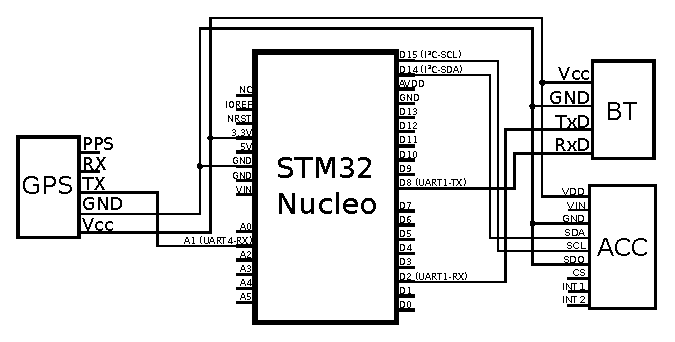
\includegraphics[scale=1.1]{img/schema.eps}
\caption{Schéma připojení periferních zařízení}\end{figure}



\section{Komunikace mezi kitem STM32 Nucleo a~serverem}
\label{msgs}
K~přenosu informací mezi kitem STM32 Nucleo a~serverem se využívá bezdrátová technologie
Bluetooth. K~úspěšnému navázání spojení je nejprve nutné se prostřednictvím serverové aplikace
spárovat a~připojit k~černé skříňce. Jakmile je spojení vytvořeno, bude černá skříňka automatiky
odesílat zprávy o~detekovaných nárazech na server (viz podkapitola \ref{crash}).
Dále skříňka na vyžádání serveru odešle svoji aktuální polohu (\ref{gps}) nebo
data z~akcelerometru (\ref{acc}).

Zprávy zasílané černou skříňkou na server mají vždy délku jednoho řádku a~jsou ukončeny
bajty \texttt{CR+LF}.
Pokyny odesílané serverem do skříňky obsahují vždy jen jeden bajt a~neukončují se pomocí \texttt{CR+LF}.

\subsection{Zpráva o~detekovaném nárazu}
\label{crash}
Bude-li skříňkou detekován náraz, odešle černá skříňka bez jakéhokoliv vyžádání
ze strany serveru následující zprávu na server:

\begin{lstlisting}[escapeinside={(*}{*)}]
crash;[acc-x];[acc-y];[acc-z];[lat];[lon]
\end{lstlisting}

Kde:

\begin{itemize}
\item \texttt{[acc-x]}, \texttt{[acc-y]} a~\texttt{[acc-z]} jsou informace o~síle nárazu v~jednotlivých osách
získané z~akcelerometru. Síla nárazu v~každé ose je vyjádřena číslem mezi -32768
a~32767.
\item \texttt{[lat]} a~\texttt{[lon]} je zeměpisná šířka a~délka místa, kde došlo k~nárazu, ve formátu
\texttt{[-]DDMMmmmmm}, kde \texttt{DD} jsou stupně, \texttt{MM} jsou minuty a~\texttt{mmmmm} jsou stotisíciny minut.
Např. hodnota \texttt{491394359} znamená $49^\circ13,94359'$, tj. $49,232393^\circ$. Kladná hodnota znamená \textit{north} nebo \textit{east}, záporná hodnota reprezentuje
\textit{south} nebo \textit{west}. Údaj \texttt{DD} se může skládat z~1-3 číslic, délka ostatních
částí (\texttt{MM} a~\texttt{mmmmmm}) je pevná. Není-li GPS poloha k~dispozici, bude
na místě obou složek odeslána hodnota \texttt{0}.
\end{itemize}

Příkladem konkrétní zprávy o~nárazu odeslané na server může být:

\begin{lstlisting}[escapeinside={(*}{*)}]
crash;31054;-724;19573;491394363;163523547
\end{lstlisting}

\subsection{Získání aktuální polohy z~GPS}
\label{gps}
Server může dále požádat černou skříňku o~odeslání své aktuální polohy bez toho,
aby došlo k~nárazu. Toto může být použito k~ladícím účelům, lokalizaci ztraceného
vozidla či k~zjištění polohy vozidla po nárazu v~případě, že v~době nárazu nebyla k~dispozici
aktuální GPS poloha.

Pro vyžádání aktuální polohy odešle server skříňku zprávu obsahující jediný znak \texttt{g}.
Na tento požadavek skříňka odpoví následující zprávou:

\begin{lstlisting}[escapeinside={(*}{*)}]
crash;[lat];[lon]
\end{lstlisting}

kde význam \texttt{[lat]} a~\texttt{[lon]} je totožný jako u~zprávy \ref{crash}.

\subsection{Získání aktuální hodnoty zrychlení}
\label{acc}
Obdobným způsobem mohou být i~vyčteny aktuální hodnoty z~akcelerometru. Pro získání
těchto hodnot serverová aplikace odešle do černé skříňky zprávu se znakem \texttt{a}.
Odpovědí bude zpráva ve formátu:

\begin{lstlisting}[escapeinside={(*}{*)}]
acc;[acc-x];[acc-y];[acc-z]
\end{lstlisting}

kde význam \texttt{[acc-x]}, \texttt{[acc-y]} a~\texttt{[acc-z]} je totožný jako u~zprávy \ref{crash}.

\section{Implementace černé skříňky}

Logika černé skříňky byla implementována pomocí jednoduchého stavového automatu,
který je znázorněn na obrázku \ref{automata}.



\begin{figure}[h]
\centering
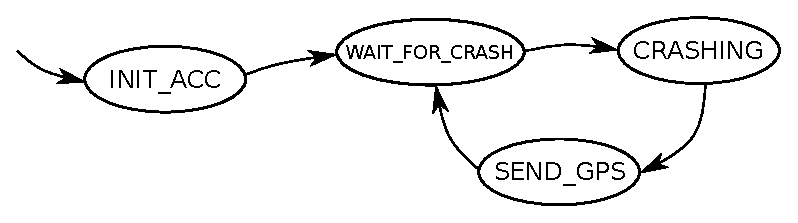
\includegraphics[scale=0.7]{img/automata.eps}
\caption{Schéma připojení periferních zařízení}\label{automata}\end{figure}



Ve výchozím stavu \texttt{INIT\_ACC} se pomocí tzv.~alive zprávy ověří funkčnost akcelerometru
a~následně dojde k~zapnutí funkce snímání zrychlení, která je ve výchozím stavu akcelerometru
po zapnutí vypnutá. Jakmile je akcelerometr inicializován, přejde automat do stavu \texttt{WAIT\_FOR\_CRASH}.

Ve stavu \texttt{WAIT\_FOR\_CRASH} se kit periodicky doptává akcelerometru na aktuální hodnotu
zrychlení ve všech třech osách. V~okamžiku, kdy hodnota zrychlení na ose \texttt{x} nebo \texttt{y}
překročí hodnotu 30000 nebo klesne pod -30000, byl detekován náraz a~automat přejde do stavu
\texttt{CRASHING}. Hodnota 30000 byla zvolena experimentálně. Nutnost detekovat
prudkou změnu směru ve směru osy \texttt{z} se nepředpokládá.

Ve stavu \texttt{CRASHING} se kit i~nadále periodicky doptává akcelerometru na aktuální zrychlení,
aby se ve zprávě odeslané na server nacházela co nejvyšší hodnota zrychlení, která
nastala, nikoliv naměřená první hodnota, která překročila prahovou úroveň.
V~tomto stavu se získané údaje porovnávají s~nejvyšší dosud zachycenou hodnotou\footnote{Při porovnání je vždy rozhodující vyšší složka z~dvojice (abs(x), abs(y))
    a~aktualizuje se vždy celá trojice (x, y, z) současně.}
i~s~prahovou hodnotou. Při překročení nejvyšší dosud naměřené hodnoty je tato hodnota
aktualizována. V~okamžiku klesnutí pod prahovou hodnotu automat přejde
do stavu \texttt{SEND\_GPS}.

Ve stavu \texttt{SEND\_GPS} kit načte aktuální polohu z~GPS a~odešle zprávu s~naměřenou hodnotou
zrychlení z~minulého kroku a~GPS souřadnicí na server. Poté se automat vrátí do stavu
\texttt{WAIT\_FOR\_CRASH}.

Implementace požadavků na aktuální GPS souřadnici nebo zrychlení ze serveru
je řešena pomocí přerušení. V~případě žádosti o~zrychlení jsou vráceny data,
které byly naposledy získány při čtení dat z~akcelerometru ve stavu \texttt{WAIT\_FOR\_CRASH}
nebo \texttt{CRASHING}. V~případě žádosti o~GPS jsou data ze senzoru čtena až v~okamžiku,
kdy jsou vyžádána.

\section{Implementace serverové aplikace pro Android}

...

\section{Autoři}

Na řešení projektu se podíleli následující autoři:

\begin{itemize}
\item Petr Rusiňák (xrusin03) -- programování kitu STM32 Nucleo, dokumentace
\item Andrej Hučko (xhucko01) -- vývoj Android aplikace
\end{itemize}

\section{Závěr}

Vytvořené řešení plní roli černé skříňky, která v~případě detekce nárazu odešle
informaci místě události a~síle nárazu na server...

TODO





\end{document}

